\documentclass{article}
\usepackage{cmap}
\usepackage[utf8]{inputenc}
\usepackage[english,ukrainian]{babel}
\usepackage{graphicx}
\usepackage{geometry}
\usepackage{listings}
\usepackage{float}
\usepackage{amsmath}
\usepackage{subfig}
\geometry{
	a4paper,
	left=20mm,
	right=20mm,
	top=15mm,
	bottom=15mm,
}
\lstset{
	language=c,
	tabsize=4,
	keepspaces,
	showstringspaces=false,
}
\graphicspath{ {./pictures} }
\setlength{\parindent}{4em}

\newcommand\subject{Архітектура комп'ютера}
\newcommand\lecturer{доцент кафедри ПЗ\\Крук О.Г.}
\newcommand\teacher{доцент кафедри ПЗ\\Крук О.Г.}
\newcommand\mygroup{ПЗ-22}
\newcommand\lab{3}
\newcommand\theme{}
\newcommand\purpose{}

\begin{document}
\begin{normalsize}
	\begin{titlepage}
		\thispagestyle{empty}
		\begin{center}
			\textbf{МІНІСТЕРСТВО ОСВІТИ І НАУКИ УКРАЇНИ\\
				НАЦІОНАЛЬНИЙ УНІВЕРСИТЕТ "ЛЬВІВСЬКА ПОЛІТЕХНІКА"}
		\end{center}
		\begin{flushright}
			\textbf{ІКНІ}\\
			Кафедра \textbf{ПЗ}
		\end{flushright}
		\vspace{200pt}
		\begin{center}
			\textbf{ЗВІТ}\\
			\vspace{10pt}
			до лабораторної роботи № \lab\\
			\textbf{на тему}: “\textit{\theme}”\\
			\textbf{з дисципліни}: “\subject”
		\end{center}
		\vspace{112pt}
		\begin{flushright}
			
			\textbf{Лектор}:\\
			\lecturer\\
			\vspace{28pt}
			\textbf{Виконав}:\\
			
			студент групи \mygroup\\
			Коваленко Д.М.\\
			\vspace{28pt}
			\textbf{Прийняв}:\\
			
			\teacher\\
			
			\vspace{28pt}
			«\rule{1cm}{0.15mm}» \rule{1.5cm}{0.15mm} 2022 р.\\
			$\sum$ = \rule{1cm}{0.15mm}……………\\
			
		\end{flushright}
		\vspace{\fill}
		\begin{center}
			\textbf{Львів — 2022}
		\end{center}
	\end{titlepage}
		
	\begin{description}
		\item[Тема.] \theme.
		\item[Мета.] \purpose.
	\end{description}

	\section*{Індивідуальне завдання}
\begin{figure}[H]
		\centering
		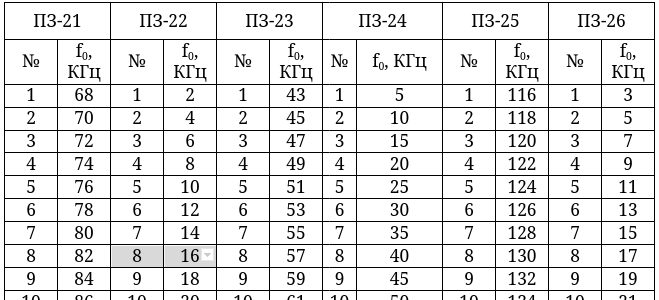
\includegraphics[scale=0.75]{v}
	\end{figure}	

	\section*{Теоретичні відомості}
	
	
	\section*{Хід роботи}
	

	\section*{Схема 1}	
	\begin{figure}[H]
		\centering
		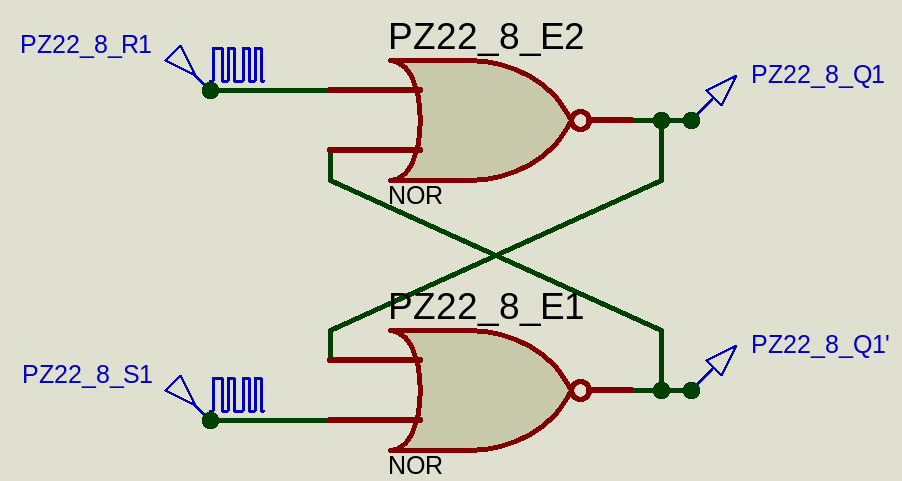
\includegraphics[scale=0.25]{s1}	
		\caption{Схема 1}
	\end{figure}

	\begin{figure}[H]
		\centering
		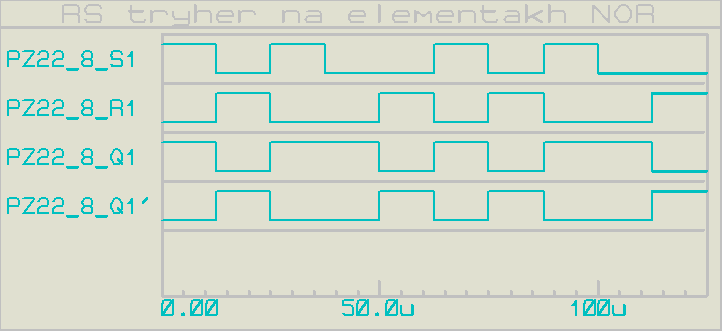
\includegraphics[scale=0.25]{g1}	
		\caption{Графік до схеми 1}
	\end{figure}

	\section*{Схема 2}	
	\begin{figure}[H]
		\centering
		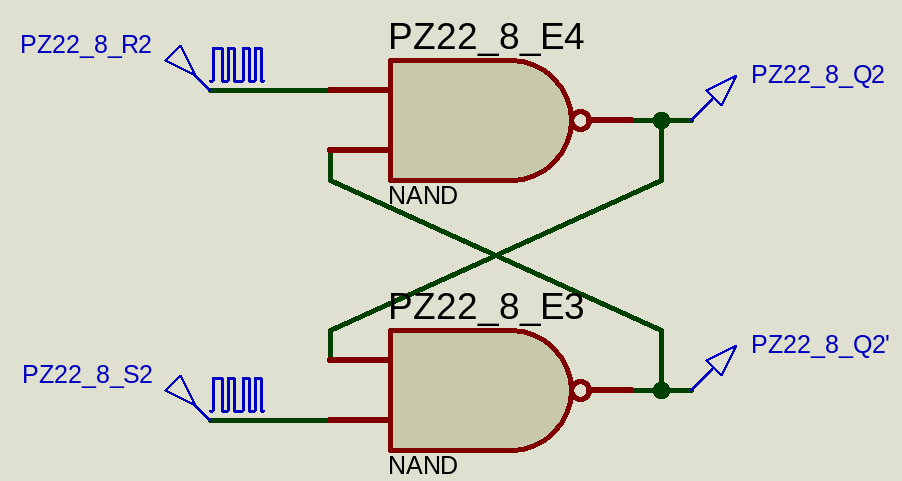
\includegraphics[scale=0.25]{s2}	
		\caption{Схема 2}
	\end{figure}
	
	\begin{figure}[H]
		\centering
		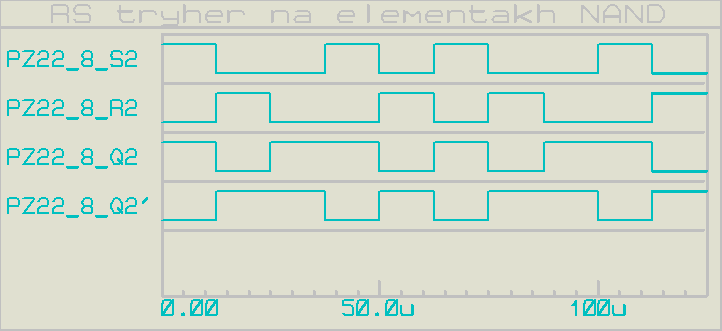
\includegraphics[scale=0.25]{g2}	
		\caption{Графік до схеми 2}
	\end{figure}

	\section*{Схема 3}	
	\begin{figure}[H]
		\centering
		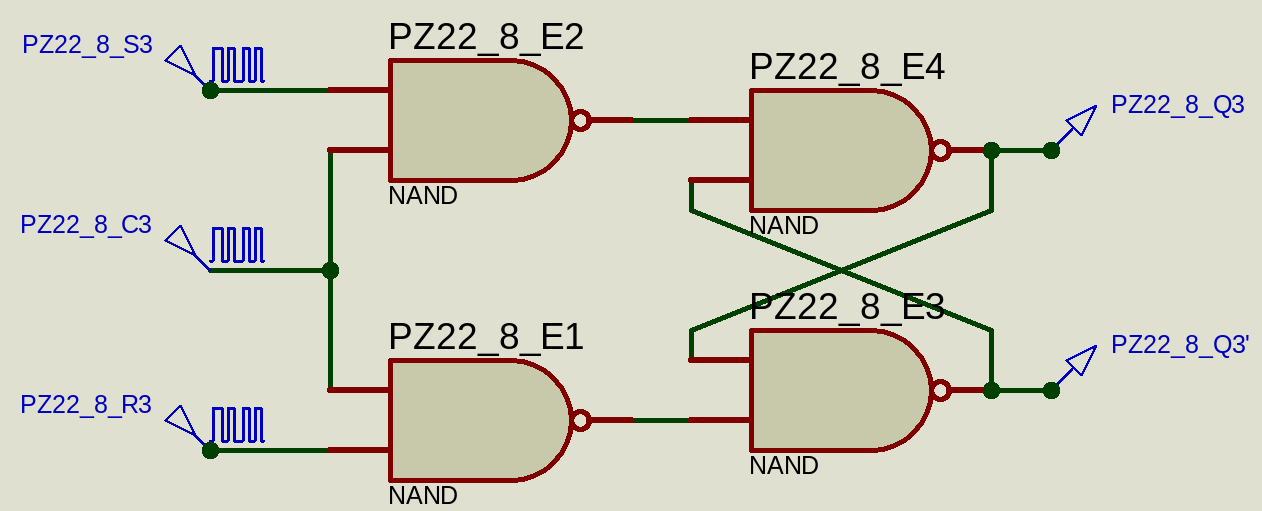
\includegraphics[scale=0.25]{s3}	
		\caption{Схема 3}
	\end{figure}
	
	\begin{figure}[H]
		\centering
		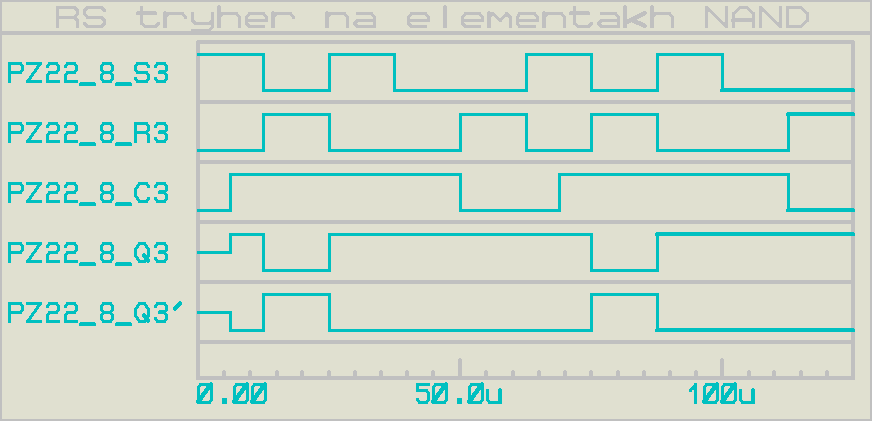
\includegraphics[scale=0.25]{g3}	
		\caption{Графік до схеми 3}
	\end{figure}

	\section*{Схема 4}	
	\begin{figure}[H]
		\centering
		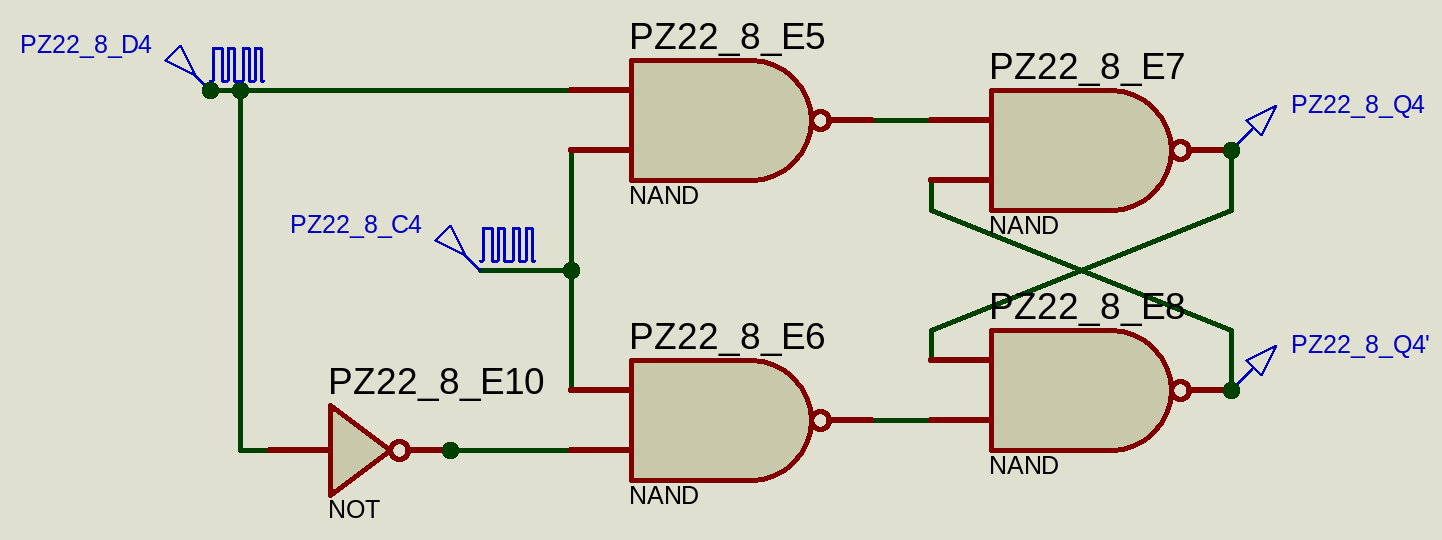
\includegraphics[scale=0.25]{s4}	
		\caption{Схема 4}
	\end{figure}
	
	\begin{figure}[H]
		\centering
		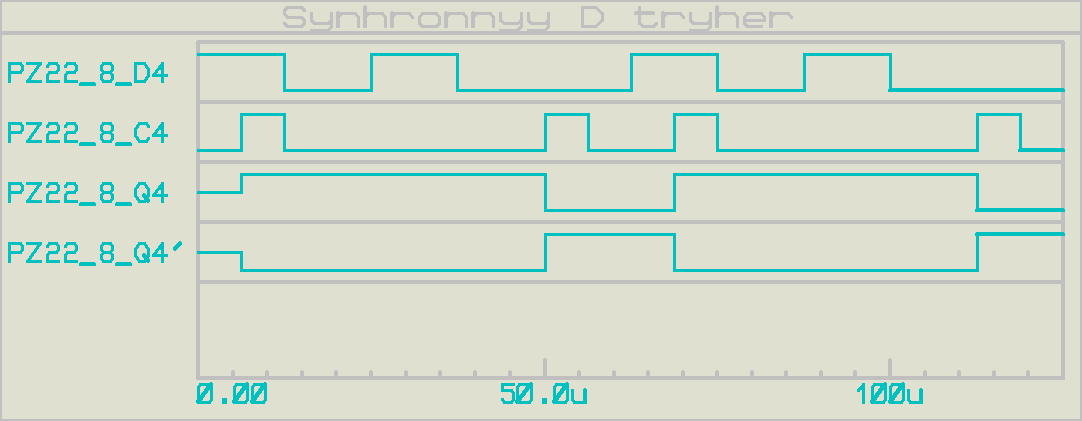
\includegraphics[scale=0.25]{g4}	
		\caption{Графік до схеми 4}
	\end{figure}

	\section*{Схема 5}	
	\begin{figure}[H]
		\centering
		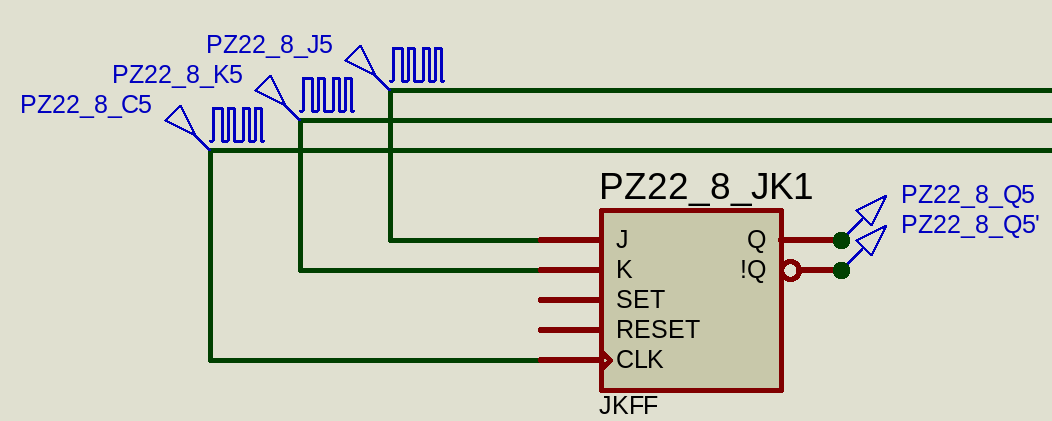
\includegraphics[scale=0.25]{s5}	
		\caption{Схема 5}
	\end{figure}
	
	\begin{figure}[H]
		\centering
		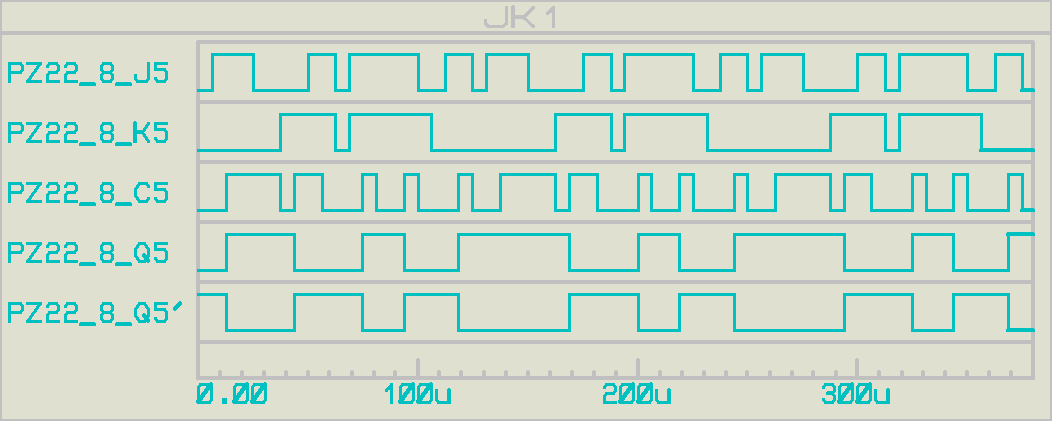
\includegraphics[scale=0.25]{g5}	
		\caption{Графік до схеми 5}
	\end{figure}

	\section*{Схема 6}	
	\begin{figure}[H]
		\centering
		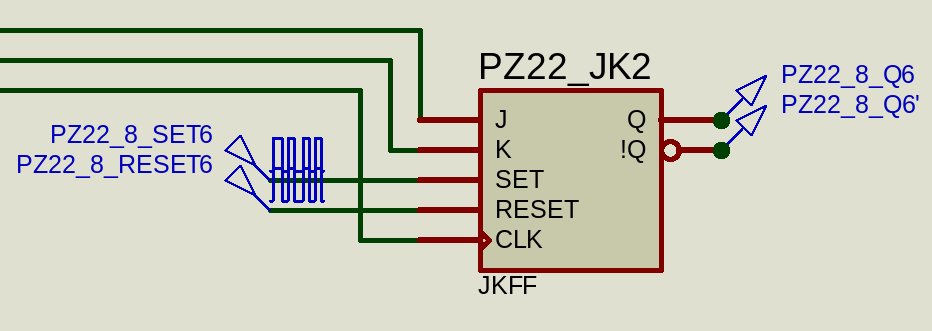
\includegraphics[scale=0.25]{s6}	
		\caption{Схема 6}
	\end{figure}
	
	\begin{figure}[H]
		\centering
		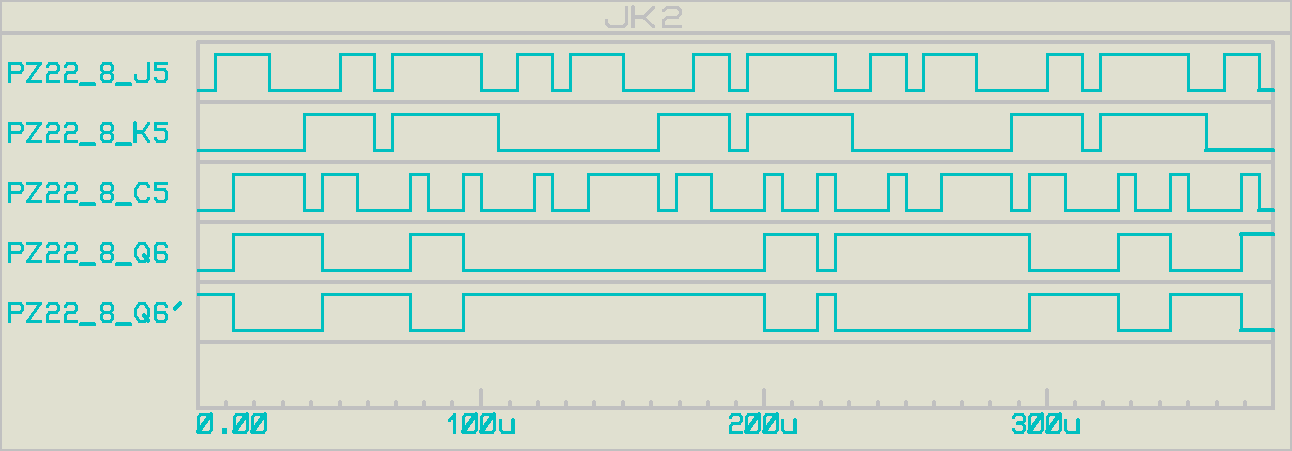
\includegraphics[scale=0.25]{g6}	
		\caption{Графік до схеми 6}
	\end{figure}

	\section*{Схема 7}	
	\begin{figure}[H]
		\centering
		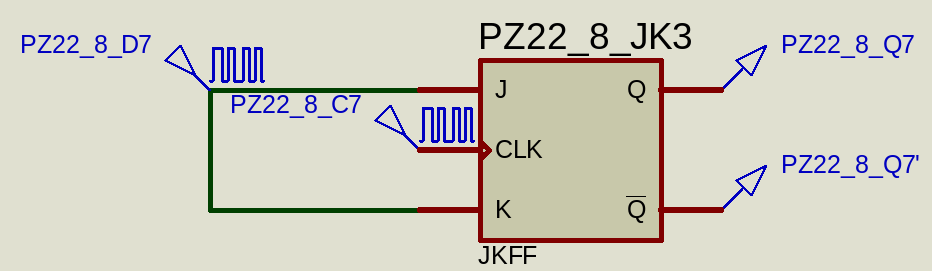
\includegraphics[scale=0.25]{s7}	
		\caption{Схема 7}
	\end{figure}
	
	\begin{figure}[H]
		\centering
		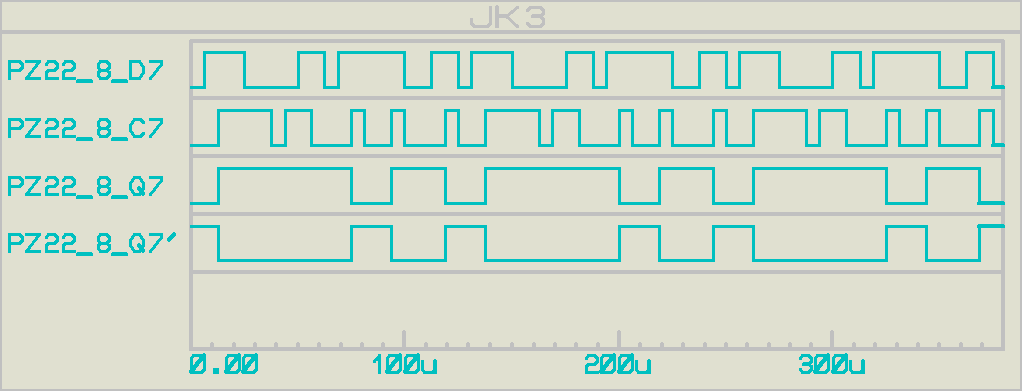
\includegraphics[scale=0.25]{g7}	
		\caption{Графік до схеми 7}
	\end{figure}

	\section*{Схема 8}	
	\begin{figure}[H]
		\centering
		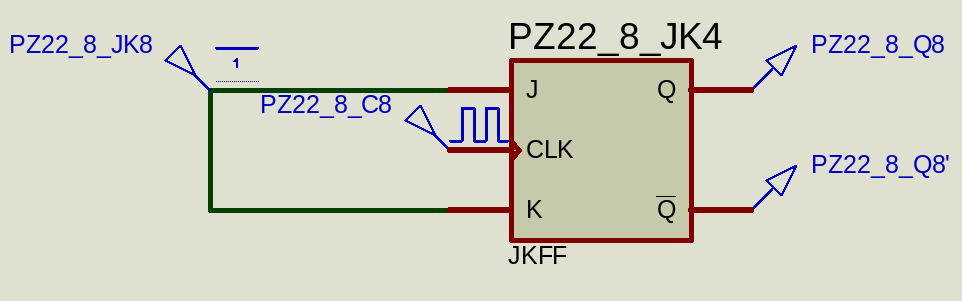
\includegraphics[scale=0.25]{s8}	
		\caption{Схема 8}
	\end{figure}
	
	\begin{figure}[H]
		\centering
		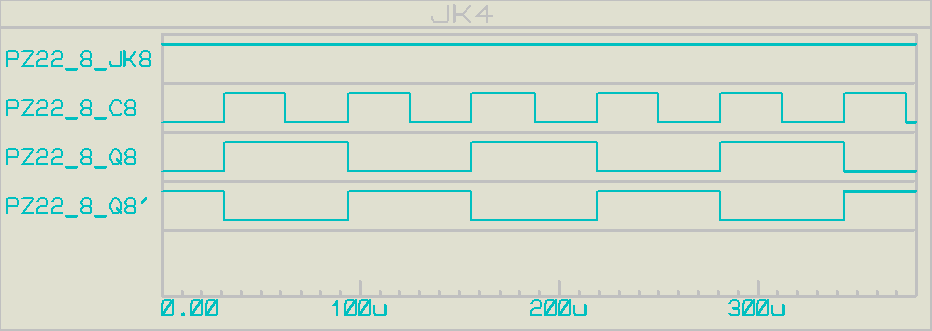
\includegraphics[scale=0.25]{g8}	
		\caption{Графік до схеми 8}
	\end{figure}

	\section*{Висновки}
	
	    
\end{normalsize}
\end{document}
